\documentclass[11pt]{article}

\usepackage[letterpaper,margin=1in]{geometry}
\usepackage[T1]{fontenc}
\usepackage[utf8]{inputenc}
\usepackage{helvet}
\renewcommand{\familydefault}{\sfdefault}
\usepackage{xcolor}
\usepackage{graphicx}
\usepackage{titlesec}
\usepackage{enumitem}
\usepackage{array}
\usepackage{tabularx}
\usepackage{longtable}
\usepackage{colortbl}
\usepackage{tcolorbox}
\usepackage{fancyhdr}
\usepackage{amsmath}
\usepackage{amssymb}
\usepackage{caption}
\usepackage{tikz}
\usetikzlibrary{arrows.meta,positioning,shapes.geometric,fit,calc}
\usepackage[hidelinks]{hyperref}

% ---- palette ----
\definecolor{navy}{HTML}{1B2A4A}
\definecolor{navytwo}{HTML}{24395F}
\definecolor{gold}{HTML}{B8860B}
\definecolor{slate}{HTML}{55606E}
\definecolor{fgreen}{HTML}{3C6E47}
\definecolor{fred}{HTML}{8A3030}
\definecolor{tblhead}{HTML}{EAEEF5}
\definecolor{tblborder}{HTML}{D5DBE5}
\definecolor{callfill}{HTML}{F3F5F9}
\definecolor{callborder}{HTML}{C7D0DE}
\definecolor{bodytext}{HTML}{1A1A1A}

\titleformat{\section}{\color{navy}\Large\bfseries}{\thesection.}{0.5em}{}
\titleformat{\subsection}{\color{navytwo}\large\bfseries}{\thesubsection}{0.6em}{}
\titleformat{\subsubsection}{\color{navytwo}\normalsize\bfseries}{\thesubsubsection}{0.6em}{}
\titlespacing*{\section}{0pt}{10pt}{4pt}
\titlespacing*{\subsection}{0pt}{9pt}{3pt}
\captionsetup{font=small,labelfont={bf,color=navy},labelsep=period,skip=4pt,position=below}

\pagestyle{fancy}
\fancyhf{}
\renewcommand{\headrulewidth}{0pt}
\renewcommand{\footrulewidth}{0pt}
\fancyfoot[C]{\color{slate}\small Financial Statement Simulator \;|\; Full proposal \;|\; page \thepage}

\newcommand{\lead}[2]{\par\addvspace{5pt}\textbf{\textcolor{#1}{#2}}}
\newcommand{\headtext}[1]{\textcolor{navy}{\textbf{#1}}}
\newcommand{\pass}{\textcolor{fgreen}{\textbf{PASS}}}
\newcommand{\provisional}{\textcolor{gold}{\textbf{PROVISIONAL}}}
\newcommand{\todo}{\textcolor{fred}{\textbf{TO VALIDATE}}}
\arrayrulecolor{tblborder}
\setlength{\tabcolsep}{4pt}
\setlength{\parskip}{0pt}
\setlength{\parindent}{1.7em}
\setlist[itemize]{leftmargin=1.4em,itemsep=2pt,topsep=2pt}
\setlist[enumerate]{leftmargin=1.7em,itemsep=2pt,topsep=2pt}

\begin{document}
\color{bodytext}

% ===== Title block =====
\begin{flushleft}
{\color{gold}\bfseries PROJECT PROPOSAL}\\[3pt]
{\color{navy}\bfseries\fontsize{26}{30}\selectfont Financial Statement Simulator}\\[4pt]
{\color{slate}\large A readable, auditable prototype for turning annual reports into scenario statements}\\[6pt]
{\color{slate}\small Prepared by Jaebum (Albert) Chung \quad | \quad Prepared for Chak \quad | \quad Status: full proposal \quad | \quad August 2026}\\[3pt]
{\color{slate}\small Internship window: 31 August 2026 to 26 February 2027}
\end{flushleft}
\vspace{4pt}
{\color{gold}\rule{\linewidth}{2pt}}
\vspace{6pt}

% ===== 1. Executive summary =====
\section{Executive summary}
The proposal is for a controlled prototype that starts with a company's annual report and produces next-period financial statements under explicit scenarios. The output keeps the firm's own line items and accounting standard. The prototype is not a point-forecasting product and does not claim that an LLM can infer economic equivalence reliably on its own.

The central design is a sequence of five separate jobs:
\begin{enumerate}
  \item read the document into rows, values, periods, units, and signs;
  \item check the printed arithmetic before assigning meaning to the row names;
  \item map each row to an accounting concept, retaining the source standard;
  \item map concepts to a small, reviewed set of economic roles used by the simulator;
  \item advance the accounting balances through explicit flows and render the result in native lines.
\end{enumerate}

The distinction between the last three jobs is important. A US GAAP line called ``Net sales'' and an IFRS line called ``Revenue'' may both receive the simulator role \texttt{revenue}, because the same scenario driver may affect both. That role assignment is a behavioural decision. It does not assert that the two accounting concepts are identical, and it does not erase the original standard-specific concepts.

The current reference build demonstrates four mechanical properties on Apple, Microsoft, SAP, and Spotify: PDF-only accepted cells match tagged ground truth on 994 of 994 cells; encode and decode reproduce 1,162 statement cells exactly, with disclosed exceptions for filer-rounded subtotals; and six scenarios with 500 paths per firm preserve the accounting identities on all 12,000 paths. The build does not yet establish that arbitrary native labels are mapped to the correct standard concept or that the hand-authored scenario responses are calibrated forecasts. Those are the principal validation tasks in the proposed work.

The requested outcome is an MVP that an accountant can inspect line by line, that refuses to simulate when a material mapping is uncertain, and that records enough evidence for another person to reproduce every accepted input, mapping decision, posting, and output.

\begin{tcolorbox}[colback=callfill,colframe=callborder,title=What this proposal asks to prove]
\begin{itemize}
  \item A PDF statement can be read with a measured abstention and error policy.
  \item A resolved statement can be represented and re-rendered without losing its native presentation.
  \item A scenario can change stocks only through named, balanced flows.
  \item Standard-specific accounting concepts can be connected to shared behavioural roles through reviewed rules, with explicit refusal when equivalence is not supported.
\end{itemize}
\end{tcolorbox}

\tableofcontents

% ===== 2. Decision and scope =====
\section{Decision, scope, and terminology}
\label{sec:scope}
\subsection{The decision the prototype supports}
A credit, research, or portfolio analyst can ask: ``Given the latest filed statements, what internally consistent statements result if demand falls, rates rise, or competition compresses margins?'' Today this is commonly answered in a spreadsheet built for one firm. The proposed tool makes the data-reading and accounting-control parts reusable, while leaving scenario assumptions visible and adjustable.

The MVP is an analytical aid. It is not a regulatory capital model, a security-pricing model, or a claim of superior point forecasts. Its stochastic output is a distribution produced by explicit scenario rules and seeded noise. A later, conditional phase may estimate a joint distribution from historical data, but that phase starts only after the mechanical and review gates pass.

\subsection{Terms used in this proposal}
An \emph{annual report} is the source document. A \emph{structured statement} is a table of rows, where every value has a label, period, unit, scale, sign convention, and location in the statement. A \emph{standard concept} is an identifier from US GAAP or IFRS, such as a revenue or receivables concept. A \emph{behavioural role} is a reviewed category that tells the simulator how a concept may respond, such as revenue, inventory, debt, or dividends.

The phrase \emph{accounting state} means the balances and flow variables needed to advance the statements. It is deliberately not called an econometric state-space model in the main text. A statistical state-space model describes a latent process and observations. This prototype first constructs an accounting state, then applies scenario equations to it. The two ideas can be combined later, but they are not the same object.

An \emph{XBRL tag} is the machine-readable fact supplied with many public filings \cite{xbrl21}. A \emph{mapping record} is the reviewable JSON record that stores a document hash, extracted pages, concept choices, role choices, adjudications, and sign-off. A \emph{born-digital PDF} is electronically generated; a scanned page, including an OCR scan, is outside the MVP because all text readers would inherit the same guessed characters.

% ===== 3. Current prototype =====
\section{What exists today}
\label{sec:status}
The repository contains a working reference implementation and committed output artifacts. The status below is intentionally more conservative than a product readiness claim.

\begin{center}
\renewcommand{\arraystretch}{1.15}
\begin{tabularx}{\linewidth}{>{\raggedright\arraybackslash}p{3.2cm} >{\raggedright\arraybackslash}p{2.2cm} X}
\hline
\rowcolor{tblhead} \headtext{Component} & \headtext{Status} & \headtext{What the evidence means} \\ \hline
PDF row extraction & \pass & Four-filer PDF-only ablation: 994 accepted cells agree with tagged values; disagreements abstain. \\ \hline
Arithmetic validation & \pass & Subtotals, assets equals liabilities plus equity, and cash continuity are checked before semantic mapping. \\ \hline
Representation and rendering & \pass & 1,162 cells round-trip exactly in the reference build; filer-rounded subtotals are retained when recomputation would alter the printed value. \\ \hline
Balanced-flow engine & \pass & Symbolic closure and acyclicity pass for the four-filer build; 12,000 simulated paths have zero identity violations. \\ \hline
Standard concept mapping & \provisional & A ladder and mapping artifacts exist, but the broader IR validation report records material concept mismatches. This layer requires correction and review before a coverage claim. \\ \hline
Behavioural role mapping & \provisional & A deterministic role table exists and drives the prototype. Coverage and sector-specific meaning are not yet validated outside the current set. \\ \hline
Scenario realism & \provisional & Directional tests pass. Parameters are authored assumptions, not calibrated forecasts. \\ \hline
\end{tabularx}
\end{center}

This table separates a mechanical guarantee from a semantic judgement. If a PDF reader disagrees, the system can abstain. If ``trade receivables'' might include several economic components, arithmetic cannot decide the correct role; that decision needs standard-aware evidence and review.

% ===== 4. Worked walkthrough =====
\section{Worked walkthrough: Apple from filing to simulation}
\label{sec:walkthrough}
This section answers the main implementation question directly. The input is Apple's 2025 Form 10-K. The reference artifacts are \texttt{out/overlay.json} and the acceptance outputs under \texttt{out/\allowbreak acceptance/\allowbreak apple/}. The following is the path one line takes.

\begin{figure}[h]
\centering
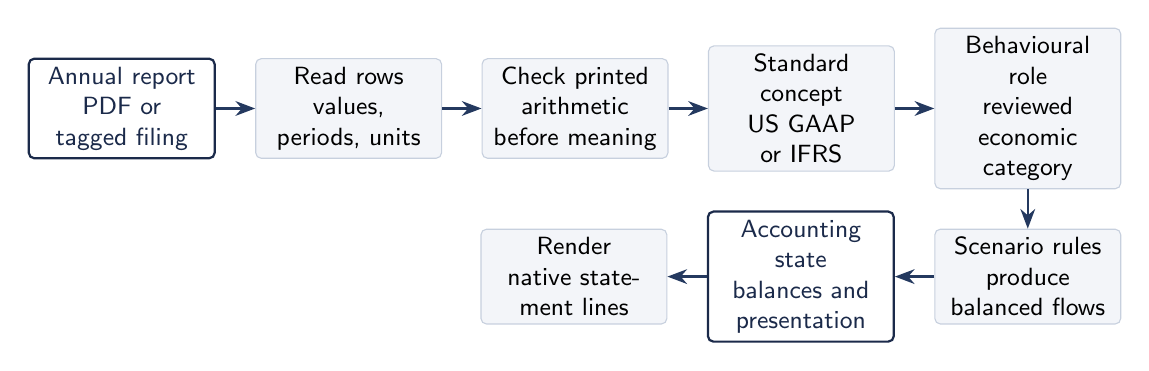
\begin{tikzpicture}[
  font=\small,
  node distance=5mm and 5mm,
  box/.style={draw=callborder, fill=callfill, rounded corners=2pt, minimum height=10mm, text width=2.15cm, inner sep=3pt, align=center},
  data/.style={draw=navy, thick, fill=white, rounded corners=2pt, minimum height=10mm, text width=2.15cm, inner sep=3pt, align=center, text=navy},
  arrow/.style={-{Stealth[length=2.5mm]}, thick, color=navytwo}
]
\node[data] (pdf) {Annual report\\PDF or tagged filing};
\node[box, right=of pdf] (read) {Read rows\\values, periods, units};
\node[box, right=of read] (check) {Check printed arithmetic\\before meaning};
\node[box, right=of check] (concept) {Standard concept\\US GAAP or IFRS};
\node[box, right=of concept] (role) {Behavioural role\\reviewed economic category};
\node[box, below=of role] (flows) {Scenario rules\\produce balanced flows};
\node[data, left=of flows] (state) {Accounting state\\balances and presentation};
\node[box, left=of state] (render) {Render\\native statement lines};
\draw[arrow] (pdf) -- (read);
\draw[arrow] (read) -- (check);
\draw[arrow] (check) -- (concept);
\draw[arrow] (concept) -- (role);
\draw[arrow] (role) -- (flows);
\draw[arrow] (flows) -- (state);
\draw[arrow] (state) -- (render);
\end{tikzpicture}
\caption{The prototype separates PDF reading, concept mapping, role mapping, and simulation. Each stage has its own evidence and refusal policy.}
\label{fig:plainpipeline}
\end{figure}

\subsection{Step 1: read the PDF}
The PDF reader uses word positions and two independent text extraction engines. It normalizes parentheses, scale headers, signs, and periods, then compares the resulting cells. A value is accepted only under the agreement rule; otherwise it is flagged. When tagged facts exist, the tag path supplies a separate reference and is used to measure the PDF-only path, not to hide its errors.

\subsection{Step 2: verify arithmetic before assigning concepts}
The reader first checks relationships that are visible in the printed numbers. For example, it verifies that Apple total assets equal current plus non-current assets, that assets equal liabilities plus equity, and that beginning cash plus the cash-flow change equals ending cash. A subtotal that cannot be verified is reported as not checkable. No taxonomy lookup is needed for this step. This is the practical meaning of ``numbers confirm structure'': labels nominate likely rows, but the numbers decide whether the proposed structure closes.

\subsection{Step 3: assign a standard concept}
A resolved row is assigned a concept using the following order:
\begin{enumerate}
  \item use the filer's own tag when it is available and passes the fact checks;
  \item reuse a previously reviewed mapping for the same filer and unchanged line;
  \item search the declared standard's concepts using the label, statement, period type, sign, and calculation relationships;
  \item let an LLM rank a constrained shortlist at build time only, with the choice recorded for review;
  \item flag the row if no choice survives the checks.
\end{enumerate}

The LLM cannot create a new accounting concept, change the value read by the deterministic readers, or override a polarity or arithmetic veto. At run time no LLM client is constructed. The runtime re-reads the source, verifies its hash against the mapping record, and replays only signed choices that remain supported by a deterministic reader.

\subsection{Step 4: assign a behavioural role}
The concept is then assigned a role used by the engine. For example, Apple's tagged current-receivables concept maps to \texttt{trade receivables}; its tagged revenue concept maps to \texttt{revenue}. The role table is authored code, not an LLM output. It includes the deciding rule, such as an exact concept entry, a label rule with statement context, or a conservative default.

The role mapping is where cross-standard comparison happens. It is not a conversion of the filing from IFRS to US GAAP. The original concept, sign, unit, and native label remain in the presentation record. The role is an additional pointer used to select a law of motion. If the line is too aggregated or its composition is unclear, the safe choice is a more general role or refusal, not an invented equivalence.

\subsection{Step 5: turn a scenario into flows}
For Apple's recession scenario, the current reference run draws lower revenue growth. Revenue leaves move first. Receivables, inventory, and payables then move through working-capital rules. Depreciation, capital expenditure, debt, dividends, buybacks, share-based compensation, investments, and cash are posted as explicit flows. The journal for the median recession path records, among other entries, a USD 334 million release from accounts receivable, USD 15.4 billion of dividends, USD 51.3 billion of buybacks, and a USD 302 million net cash decrease. Each flow has at least two accounting legs, so the engine does not need a balancing plug.

The updated values are rendered under Apple's native labels. In the committed output, net sales move from 416,161 to 412,665 million, accounts receivable move from 39,777 to 39,443 million, and the receivables cash-flow line is 334 million. The point of the example is traceability: the reader can follow the source row, its concept, its role, its flow, and its output without reading the implementation.

% ===== 5. Mapping =====
\section{How accounting concepts become shared economic meaning}
\label{sec:mapping}
\subsection{Why one name is not enough}
Accounting labels are not a universal dictionary. ``Revenue'', ``net sales'', ``turnover'', and ``net interest income'' can refer to different scopes. Conversely, two firms can use different words for a similar operating balance. Industry context, statement location, period type, sign, calculation relationships, and note definitions all matter.

The prototype therefore stores two mappings and never treats a label match as proof of economic identity:
\begin{center}
\renewcommand{\arraystretch}{1.2}
\begin{tabularx}{\linewidth}{>{\raggedright\arraybackslash}p{3.3cm} X X}
\hline
\rowcolor{tblhead} \headtext{Layer} & \headtext{Question answered} & \headtext{Evidence and failure policy} \\ \hline
Accounting concept & Which standard-defined fact does this printed row represent? & Tags, standard-scoped candidates, period/sign/footing checks, prior review, constrained LLM shortlist. Unresolved material rows are flagged. \\ \hline
Behavioural role & Which law of motion should act on that concept in this simulation? & Authored role table, statement context, calculation hierarchy, and reviewer sign-off. Ambiguous or unsupported roles cause refusal or conservative holding. \\ \hline
\end{tabularx}
\end{center}

\subsection{Worked cross-standard mapping}
The following is the intended form of a reviewed mapping record. It shows shared behaviour without claiming that the concepts or disclosure scopes are identical.

\begin{center}
\renewcommand{\arraystretch}{1.15}
\begin{tabularx}{\linewidth}{>{\raggedright\arraybackslash}p{2.6cm} >{\raggedright\arraybackslash}p{2.1cm} >{\raggedright\arraybackslash}p{4.1cm} X}
\hline
\rowcolor{tblhead} \headtext{Printed line} & \headtext{Framework} & \headtext{Concept record} & \headtext{Role used by engine} \\ \hline
Net sales & US GAAP & Filer's tagged revenue concept, subject to statement context & Revenue \\ \hline
Revenue & IFRS & Filer's tagged IFRS revenue concept, subject to statement context & Revenue \\ \hline
Accounts receivable, net & US GAAP & Current receivables concept on the balance sheet; cash-flow delta is a separate presentation of the movement & Trade receivables \\ \hline
Trade and other receivables & IFRS & Receivables concept only after note and calculation context confirm its composition & Receivables, or a more general operating asset role \\ \hline
\end{tabularx}
\end{center}

The last row illustrates the important boundary. If ``trade and other receivables'' includes non-trade balances that respond differently, a single receivables role may be too strong. The system can preserve the line for reporting while refusing a driver that needs a finer split. This is preferable to silently assigning an economically attractive but unsupported mapping.

\subsection{What the current evidence says}
The four-filer acceptance build validates the numeric and accounting controls after the mapping artifacts are supplied. It does not validate every concept choice. The separate IR validation report contains examples where a label was assigned to a broad, wrong-standard, or off-face concept. Those records are now treated as defects to resolve, not as evidence of successful cross-standard mapping. The proposed work adds standard-scoped validation against the filer's own tags, concept-level precision and recall, role-level reviewer agreement, and refusal tests for ambiguous lines.

% ===== 6. Component contracts =====
\section{Component contracts}
Each component is described using the same three questions: what it does, how it is designed, and why that design is needed.

\subsection{Document reader}
\textbf{What it does.} Converts a born-digital annual report into candidate statement rows and cells.\\
\textbf{How it is designed.} Word geometry, two text engines, normalization, agreement gates, and arithmetic identities run in sequence. Tagged facts are a separate path when present. All disagreements become flags.\\
\textbf{Why.} A PDF stores drawing instructions rather than a table object. Independent interpretations make disagreement observable, while identity checks catch some errors that happen to agree. Scanned and OCR pages are refused because their readers share a guessed text layer.

\subsection{Arithmetic validator}
\textbf{What it does.} Verifies subtotal addition, assets equals liabilities plus equity, cash continuity, and per-share checks where available.\\
\textbf{How it is designed.} Labels propose candidate totals and children. The validator searches only simple signed relationships and requires closure across reported columns, with a decimals-based rounding tolerance. It reports ``not checkable'' when an anchor is absent.\\
\textbf{Why.} Arithmetic can validate printed structure without pretending to understand every accounting label. It must run before semantic mapping so a plausible concept cannot rescue a table that does not close.

\subsection{Concept mapper}
\textbf{What it does.} Gives each accepted row a standard concept and records the evidence.\\
\textbf{How it is designed.} The mapping ladder is standard-scoped, uses the filer's tags and prior reviewed records first, constrains any LLM to candidate concepts, applies period/sign/statement checks, and requires sign-off for residual choices.\\
\textbf{Why.} Different standards and industries use overlapping labels. A model can help search and explain candidates, but it should not be the source of an unconstrained ontology decision. The artifact makes the decision reviewable and keeps runtime deterministic.

\subsection{Behaviour layer}
\textbf{What it does.} Connects standard concepts to the economic categories consumed by the scenario and accounting engine.\\
\textbf{How it is designed.} A versioned, hand-authored table assigns roles such as revenue, receivables, inventory, debt, depreciation, dividends, and cash-flow movements. The deciding rule and any fallback are recorded. A role can inherit through a calculation hierarchy only when the economic interpretation is safe.\\
\textbf{Why.} The engine should not contain a separate implementation for every spelling or standard. At the same time, shared behaviour must remain an explicit modelling assumption rather than a hidden semantic claim.

\subsection{Accounting state and renderer}
\textbf{What it does.} Stores the values needed to advance the statements and reconstructs the firm's native presentation.\\
\textbf{How it is designed.} Leaf balances are stored by concept, dimensions, period role, and column. Row labels, order, units, signs, precision, and derivation relationships are stored in a presentation record. Derived totals are recomputed where the filing's relationships support it; filer-rounded totals remain stored when necessary.\\
\textbf{Why.} A common representation is useful for shared rules, but a fixed template would discard firm-specific lines. The variable-width representation preserves each firm's disclosed shape while giving common concepts common coordinates.

\subsection{Flow engine}
\textbf{What it does.} Produces next-period balances and cash flows without a balancing plug or circular calculation.\\
\textbf{How it is designed.} The period order is income, operating-stock targets, discretionary schedules, closing flows, liquidity policy, derived totals, and validation. Every flow posts balanced debit and credit effects. Cash is the result of explicit cash postings, not a residual. Symbolic balance and dependency checks run before numeric simulation.\\
\textbf{Why.} A residual plug can hide a missing or double-counted movement. An explicit journal makes the cause of every change inspectable and makes the accounting identity an invariant of the engine.

\subsection{Scenario layer}
\textbf{What it does.} Converts scenario inputs into changes in roles and flows.\\
\textbf{How it is designed.} The MVP uses authored responses to GDP growth, inflation, short rates, competition, and firm demand, with seeded noise. Common random numbers make scenario differences comparable.\\
\textbf{Why.} The prototype must be executable before a calibrated historical dataset exists. The tradeoff is explicit: directional credibility is tested now; probability calibration is deferred to Part II.

% ===== 7. Evidence =====
\section{Prototype evidence and limitations}
\label{sec:evidence}
\subsection{Measured results}
The acceptance report records the following results for Apple and Microsoft under US GAAP and SAP and Spotify under IFRS.

\begin{center}
\renewcommand{\arraystretch}{1.15}
\begin{tabularx}{\linewidth}{>{\raggedright\arraybackslash}p{4cm} >{\raggedright\arraybackslash}p{2cm} X}
\hline
\rowcolor{tblhead} \headtext{Test} & \headtext{Result} & \headtext{Interpretation} \\ \hline
PDF-only extraction & 994/994 accepted cells match tags & Zero observed accepted-cell errors on this four-filer set; the 95 percent rule-of-three upper bound is 0.30 percent for this sample \cite{ruleofthree}. \\ \hline
Encode and render & 1,162/1,162 cells exact & The representation preserves the tested rows and presentation. This does not prove that every concept choice is correct. \\ \hline
Arithmetic & All tested subtotal and identity checks pass & Printed rounding is tolerated and reported. \\ \hline
Simulation integrity & 0 identity violations on 12,000 paths & The engine adds no imbalance to the filer's base residual. \\ \hline
Directional tests & All required signs pass for four filers & This tests response direction, not forecast calibration or causal truth. \\ \hline
Semantic mapping across arbitrary IR reports & Not validated & The IR report contains material concept mismatches and is the first correction target. \\ \hline
\end{tabularx}
\end{center}

\subsection{Known limitations}
The tested firms are not a representative industry sample. Financial institutions, energy businesses, insurers, and firms with highly specialized presentation are not yet covered by the same role recipes. The untagged mode is restricted to born-digital PDFs. A concept may be extracted correctly but mapped too broadly, to the wrong standard, or to a cash-flow movement rather than a stock. A balanced simulation can therefore still be economically unhelpful if a role is wrong. The audit trail must expose that distinction.

\subsection{Prototype commands and artifacts}
The current workflow has two modes:
\begin{itemize}
  \item build time: \texttt{python -m fss onboard <pdf>} reads the document, permits bounded LLM assistance, and emits a reviewable mapping record;
  \item run time: \texttt{python -m fss runtime <pdf>} checks the document hash, re-reads it deterministically, replays signed decisions, and refuses drift or unresolved material cells.
\end{itemize}

For the Apple example, the accounting representation is in \texttt{out/overlay.json}. The acceptance summary is in \texttt{out/\allowbreak acceptance/\allowbreak apple/\allowbreak outcome.json}; the recession journal is in \texttt{out/\allowbreak acceptance/\allowbreak apple/\allowbreak journal\_recession.json}; and the rendered statements are in \texttt{out/\allowbreak acceptance/\allowbreak apple/\allowbreak simulated\_recession.md}. These are the prototype artifacts to show in the review. A reviewer can inspect the exact rows and postings instead of relying on a readiness label.

% ===== 8. Proposed build and acceptance =====
\section{Proposed build and acceptance gates}
\label{sec:plan}
The first phase is evidence correction and reviewer workflow, not a larger model. The work is organized around the unresolved risks.

\begin{enumerate}
  \item \textbf{Immediate safety hardening, now.} The code now rejects a signed artifact that names the wrong reporting standard, refuses unsigned or legacy artifacts at runtime, records row-level mapping provenance, and refuses simulation when material semantics or cash-flow bindings are unresolved. These are correctness fixes, not claims of universal semantic understanding.
  \item \textbf{Claim and artifact audit, 2 weeks.} Reconcile every existing mapping artifact with the declared standard and the filer's tags. Separate stock concepts from cash-flow movements, identify company extensions, and classify each mismatch as a reader error, wrong standard, wrong statement, granularity mismatch, or legitimate extension. Produce a concept-level precision and recall report.
  \item \textbf{Reviewed semantic MVP, 3 weeks.} Select one or two cohorts (technology/software is the initial candidate). Display standard-scoped candidates with statement location, period type, balance, units, dimensions, calculation parents, and note evidence. Let an LLM rank this shortlist at build time, but require a reviewer to accept, change, split, hold, or refuse each material mapping. Add regression cases for shared labels, extensions, aggregated receivables, and stock-versus-flow collisions.
  \item \textbf{Role recipes and prototype hardening, 3 weeks.} Define reviewer-approved behavioural-role recipes for the selected cohorts, including revenue, COGS, receivables, inventory, payables, debt, leases, and cash-flow articulation. Keep unresolved rows in the report, but do not let broad defaults drive a simulation. Stabilize source-hash checking, round-trip tests, and the flow journal before expanding coverage.
  \item \textbf{Scenario review, 2 weeks.} Put every driver, coefficient, law of motion, and refusal condition in a review table. Test only directional response and broad plausibility at MVP stage. State clearly that these are authored assumptions, not calibrated probabilities.
  \item \textbf{Conditional calibration, research extension.} If the semantic MVP gates pass and a historical panel is available, estimate and backtest a conditional joint distribution of drivers. Compare it with the authored rules; never use calibration to compensate for failed extraction or mapping.
\end{enumerate}

\subsection{Acceptance gates for the MVP}
\begin{enumerate}
  \item Accepted extraction cells have zero observed errors against an independently verified reference on the agreed gating set; all other cells are flagged.
  \item The declared standard and the concept choice agree with the filer's tag or a documented reviewer decision; wrong-standard and off-face choices are counted as failures.
  \item The rendered statement preserves labels, order, values, signs, units, periods, and precision, with filer-rounded subtotals explicitly disclosed.
  \item Every simulated path preserves the base accounting residual and has no additional imbalance or cash discontinuity.
  \item Required role assignments are complete, and an unresolved material role refuses simulation.
  \item The selected cohort meets a pre-specified mapping bar (concept agreement with tagged facts where available, reviewer agreement for residuals, and zero wrong-standard replay).
  \item Scenario direction, bounded growth, margins, non-negative stocks, and representative accountant review pass. This is a directional-credibility gate, not a forecast-accuracy claim.
\end{enumerate}

% ===== 9. Governance =====
\section{Governance, risks, and open decisions}
\label{sec:governance}
\subsection{Controls}
Every run records the source hash, code version, mapping-record hash, standard declaration, reader outputs, flags, reviewer decisions, scenario configuration, random seed, flow journal, and validation results. The runtime does not construct an LLM client. A changed source requires re-onboarding and sign-off. This supports effective challenge and reproducibility in the sense expected by SR 11-7 \cite{sr117} and the data-integrity principles of BCBS 239 \cite{bcbs239}.

\subsection{Risk register}
\begin{center}
\renewcommand{\arraystretch}{1.15}
\begin{tabularx}{\linewidth}{>{\raggedright\arraybackslash}p{4.1cm} >{\raggedright\arraybackslash}p{1.6cm} X}
\hline
\rowcolor{tblhead} \headtext{Risk} & \headtext{Rating} & \headtext{Control} \\ \hline
Wrong or overly broad concept mapping & High & Standard-scoped candidates, tag comparison, role-level review, materiality thresholds, and refusal. Current IR mismatches remain open until corrected. \\ \hline
PDF layout outside reader grammar & Medium & Independent readers, arithmetic checks, flags, seeded pathologies, and born-digital scope refusal. \\ \hline
Balanced but economically wrong scenario & High & Separate accounting-integrity and economic-plausibility gates; authored assumptions exposed; calibration is conditional. \\ \hline
Industry-specific vocabulary & Medium & Add a role recipe only with a worked example, reviewer sign-off, and cohort-level tests. \\ \hline
Review capacity & Medium & Batch onboarding and expand the cohort only at the rate the reviewer can sign off. \\ \hline
\end{tabularx}
\end{center}

\subsection{Open decisions}
\begin{enumerate}
  \item Which firms and industries form the first reviewer-approved gating set?
  \item What level of concept and role agreement is required before a line is allowed to drive a simulation?
  \item Which existing macro-model interface supplies scenario inputs, and who owns the industry parameters?
  \item Which outputs are sufficient for the first analyst demonstration: full native statements, selected statement sections, or both?
\end{enumerate}

% ===== Appendix A =====
\clearpage
\appendix
\section{Technical representation and accounting closure}
\label{app:technical}
This appendix gives the notation after the reader has seen the concrete workflow. Let $s$ denote a structured statement. It contains ordered rows, values, labels, periods, dimensions, units, signs, and precision. The encoder separates information-bearing values from presentation metadata:
\begin{equation}
E(s)=(z,m).
\end{equation}
Here $z$ stores leaf values keyed by concept, dimensions, and period role. The map $m$ stores row order, native labels, displayed signs, units, precision, columns, and the derivation relationships used to recompute a subtotal. The decoder $D$ renders a statement from the pair. The round-trip test is $D(E(s))=s$ on the tested domain.

The result is conditional. It proves that the representation does not lose information after a row has a concept. It does not prove that a PDF label was assigned the correct concept. That is why concept mapping has its own evidence and acceptance gate.

Let $a$ index balance-sheet accounts. Let $\beta_a$ be $+1$ for an asset account and $-1$ for a liability or equity account. Let $\phi_f(a)$ be the amount posted to account $a$ by flow $f$. A flow is balanced when:
\begin{equation}
\sum_a \beta_a\phi_f(a)=0.
\end{equation}
If the opening residual is $R_t=\sum_a\beta_a s_t(a)$ and every flow is balanced, then:
\begin{equation}
R_{t+1}=\sum_a\beta_a\left(s_t(a)+\sum_f\phi_f(a)\right)=R_t.
\end{equation}
The engine preserves the source filing's rounding residual and adds none of its own. Cash is an explicit account whose change is the sum of cash postings, so the cash-flow statement is a report of those postings rather than a residual plug.

\section{Mapping record and review protocol}
\label{app:record}
A mapping record contains the document identifier and hash, declared framework, statement page locations, each extracted row, candidate concepts, selected concept, evidence source, polarity and period attributes, selected behavioural role, role rationale, flags, adjudications, code version, and reviewer sign-off. The runtime checks the source hash and re-runs deterministic readers. A signed value is replayed only if a reader still reads that same value. Any drift or unresolved material field stops the run.

The review screen should show one row at a time with four panes: the source crop, the extracted cells, the standard concept candidates and evidence, and the proposed role and law of motion. The reviewer can accept, choose another candidate, split the role, hold the line at base value, or refuse simulation. Each action is recorded. This is the practical answer to the question ``can an LLM do the concept mapping?'' The LLM can reduce search effort; the controlled system decides only from constrained candidates and a human-approved record.

\section{Prototype walkthrough data}
\label{app:prototype}
The Apple recession example uses the following committed outputs. Monetary values are in USD millions unless otherwise stated.

\begin{center}
\renewcommand{\arraystretch}{1.15}
\begin{tabularx}{\linewidth}{>{\raggedright\arraybackslash}p{4.2cm} >{\raggedright\arraybackslash}p{2.2cm} X}
\hline
\rowcolor{tblhead} \headtext{Trace item} & \headtext{Value} & \headtext{Source or explanation} \\ \hline
Apple net sales, filed & 416,161 & Native income-statement row in the prior column of the acceptance output. \\ \hline
Apple net sales, recession path & 412,665 & Median-net-income path in \texttt{simulated\_recession.md}. \\ \hline
Accounts receivable, filed & 39,777 & Native balance-sheet row in the prior column. \\ \hline
Accounts receivable, recession path & 39,443 & Working-capital target implied by the recession path. \\ \hline
Receivables cash-flow movement & 334 & Explicit journal entry, equal to the negative stock movement under the filing's cash-flow sign convention. \\ \hline
Recession journal identity violations & 0 & Acceptance outcome for Apple; all six scenarios have zero violations. \\ \hline
\end{tabularx}
\end{center}

\begin{thebibliography}{20}\small
\bibitem{velezpareja} I.~V\'elez-Pareja and J.~Tham, ``Forecasting Financial Statements with No Plugs and No Circularity,'' \emph{The IUP Journal of Accounting Research and Audit Practices}, 2010; and I.~V\'elez-Pareja, ``To Plug or Not to Plug: A Note on Financial Statement Forecasting,'' SSRN Working Paper.
\bibitem{godley} W.~Godley and G.~Lavoie, \emph{Monetary Economics: An Integrated Approach to Credit, Money, Income, Production and Wealth}, Palgrave Macmillan, 2007.
\bibitem{penman} S.~Penman, \emph{Financial Statement Analysis and Security Valuation}, 5th ed., McGraw-Hill, 2013.
\bibitem{xbrl21} XBRL International, \emph{Extensible Business Reporting Language (XBRL) 2.1}, Recommendation, 2003.
\bibitem{calc11} XBRL International, \emph{Calculations 1.1}, Recommendation, 2023.
\bibitem{usgaap} Financial Accounting Standards Board, \emph{US GAAP Financial Reporting Taxonomy}, annual releases.
\bibitem{ifrstax} IFRS Foundation, \emph{IFRS Accounting Taxonomy}, annual releases.
\bibitem{sec33_9002} U.S. Securities and Exchange Commission, \emph{Interactive Data to Improve Financial Reporting}, Release No. 33-9002, 2009.
\bibitem{efm} U.S. Securities and Exchange Commission, \emph{EDGAR Filer Manual, Volume II}, current version.
\bibitem{esef} European Securities and Markets Authority, \emph{European Single Electronic Format Regulatory Technical Standard}, in force 2020.
\bibitem{arelle} Arelle project, \emph{An Open Source XBRL Platform}, \texttt{arelle.org}.
\bibitem{sr117} Board of Governors of the Federal Reserve System and OCC, \emph{Supervisory Guidance on Model Risk Management}, SR Letter 11-7, 2011.
\bibitem{bcbs239} Basel Committee on Banking Supervision, \emph{Principles for Effective Risk Data Aggregation and Risk Reporting}, 2013.
\bibitem{ruleofthree} B.~D. Jovanovic and P.~S. Levy, ``A Look at the Rule of Three,'' \emph{The American Statistician}, 51(2), 1997.
\bibitem{spike} KG Encoding Spike report, this repository, June 2026.
\end{thebibliography}

\end{document}
